\section{Appendices}
\begin{itemize}

\item{\textbf{Appendix 1}}

All the referred projects and the projects mentioned in the article

\item{\textbf{Appendix 2}}

Versions about Ruby on Rails

\item{\textbf{Appendix 3}}

The Python Program used to generate JSON file with an input XML file

\item{\textbf{Appendix 4}}

Internship Agreement

\item{\textbf{Appendix 5}}

Assessment Report

\end{itemize}
\newpage
\subsection{All the referred projects and the projects mentioned in the article}
\begin{enumerate}
\item{\textbf{JQuery}}

A fast, small, and feature-rich JavaScript library(\url{https://jquery.com/})

\item{\textbf{Google Map JavaScript APIs}}

Provided by Google freely, enormous APIs associated with google map(\url{https://developers.google.com/maps/documentation/javascript/tutorial}) 

\item{\textbf{Google chart}}

Provided by Google freely, enormous APIs for many different types of graphs(\url{https://developers.google.com/chart/interactive/docs/})

\item{\textbf{SWARMON}}

A second year students' project realised by Benoit BOURDON, Quentin DESCOURS, Simon STEPHAN, Mouad BICHOUARINE and Jean-Jacques BOYE, under the supervision of Olivier REYNET at ENSTA Bretagne, aims to provide a tracking system for WRSC

\item{\textbf{MYR}}

A 3rd year students' project at ENSTA Bretagne based on the SWARMON by Bastien DROUOT and Benoit BOURDON, which aims to enhance the development of web site of tracking system and create a web generator for monitoring robot(\url{https://github.com/Sylyon/MYR})

\item{\textbf{DataTable}}

A project based on the jQuery JavaScript libraries aims to create a dynamic and interacted data table with any html table(\url{http://datatables.net/})

\item{\textbf{Carrierwave}}

A gem(open source and free to use) for ruby on rails makes easier to control the uploading files to the sites based on rails framework(\url{https://github.com/carrierwaveuploader/carrierwave})

\item{\textbf{Mini\_magick}}

A light gem(open source and free to use)  and a ruby wrapper for ImageMagick or GraphicsMagick(\url{https://github.com/minimagick/minimagick})

\item{\textbf{Simple\_captcha}}

A gem(open source and free to use)  easy to add captcha into web sites based on rails framework(\url{https://github.com/galetahub/simple-captcha})

\item{\textbf{Noun}}

A project offers enormous awesome icons(\url{https://thenounproject.com/})

\item{\textbf{Favicon}}

A project offers awesome icons which could be inserted easily into html code(\url{http://fortawesome.github.io/Font-Awesome/3.2.1/examples/})

\item{\textbf{Current Web site}}

All the codes are in my Github repertoire(\url{https://github.com/nicolas2lee/AdvancedMYR}) 
\end{enumerate}
\subsection{Versions about Ruby on Rails}
Actually my work environment is ubuntu 14.04.
In order to install ruby on rails, I used rvm which is easy to control the version of ruby.
All the versions about ruby on rails for WRSC 2015 are listed below:

\begin{lstlisting}
rvm -v:

rvm 1.26.11 (latest) by Wayne E. Seguin <wayneeseguin@gmail.com>, Michal Papis <mpapis@gmail.com> [https://rvm.io/]


ruby -v:

ruby 2.1.1p76 (2014-02-24 revision 45161) [i686-linux]


rails -v:

Rails 4.2.3
\end{lstlisting}
\newpage
\subsection{The Python Program used to generate JSON file with an input XML file}
This program is which I used to generate a JSON file from a XML file during WRSC.
\begin{lstlisting}
#Author is Conny Ljunggren, Aland University of Applied Sciences - Finland
namespaces = {'gml': 'http://www.opengis.net/gml'}
import json
import xml.etree.ElementTree as ET

tree = ET.parse('XML_IfA_Sailing_2stAttempt.xml')
root = tree.getroot()

data = []
for section in root.findall('Section'):
	si = section.find('sectioni').text
	sj = section.find('sectionj').text
	timeString = section.find('dateTime').text
	timeCleaned = timeString.replace('-', '').replace('T', '').replace(':', '').replace('Z', '')
	
	position = section.find('gml:pos', namespaces).text
	latitude = float(position.split()[0])
	longitude = float(position.split()[1])
	data.append({"sectioni":si, "sectionj":sj, "position":[{"latitude":latitude, "longitude":longitude, "datetime":timeCleaned}]})

fullData = {"tracker_id":"6", "name":"IfA_Sailing", "data":data}

with open('XML_IfA_Sailing_2ndAttempt.json', 'w') as outfile:
    json.dump(fullData, outfile)
\end{lstlisting}
\subsection{Internship Agreement}

\includepdf[page=3-9]{internshipagreement.pdf}


\subsection{Assessment Report}
\begin{figure}[h!]
    \centering
    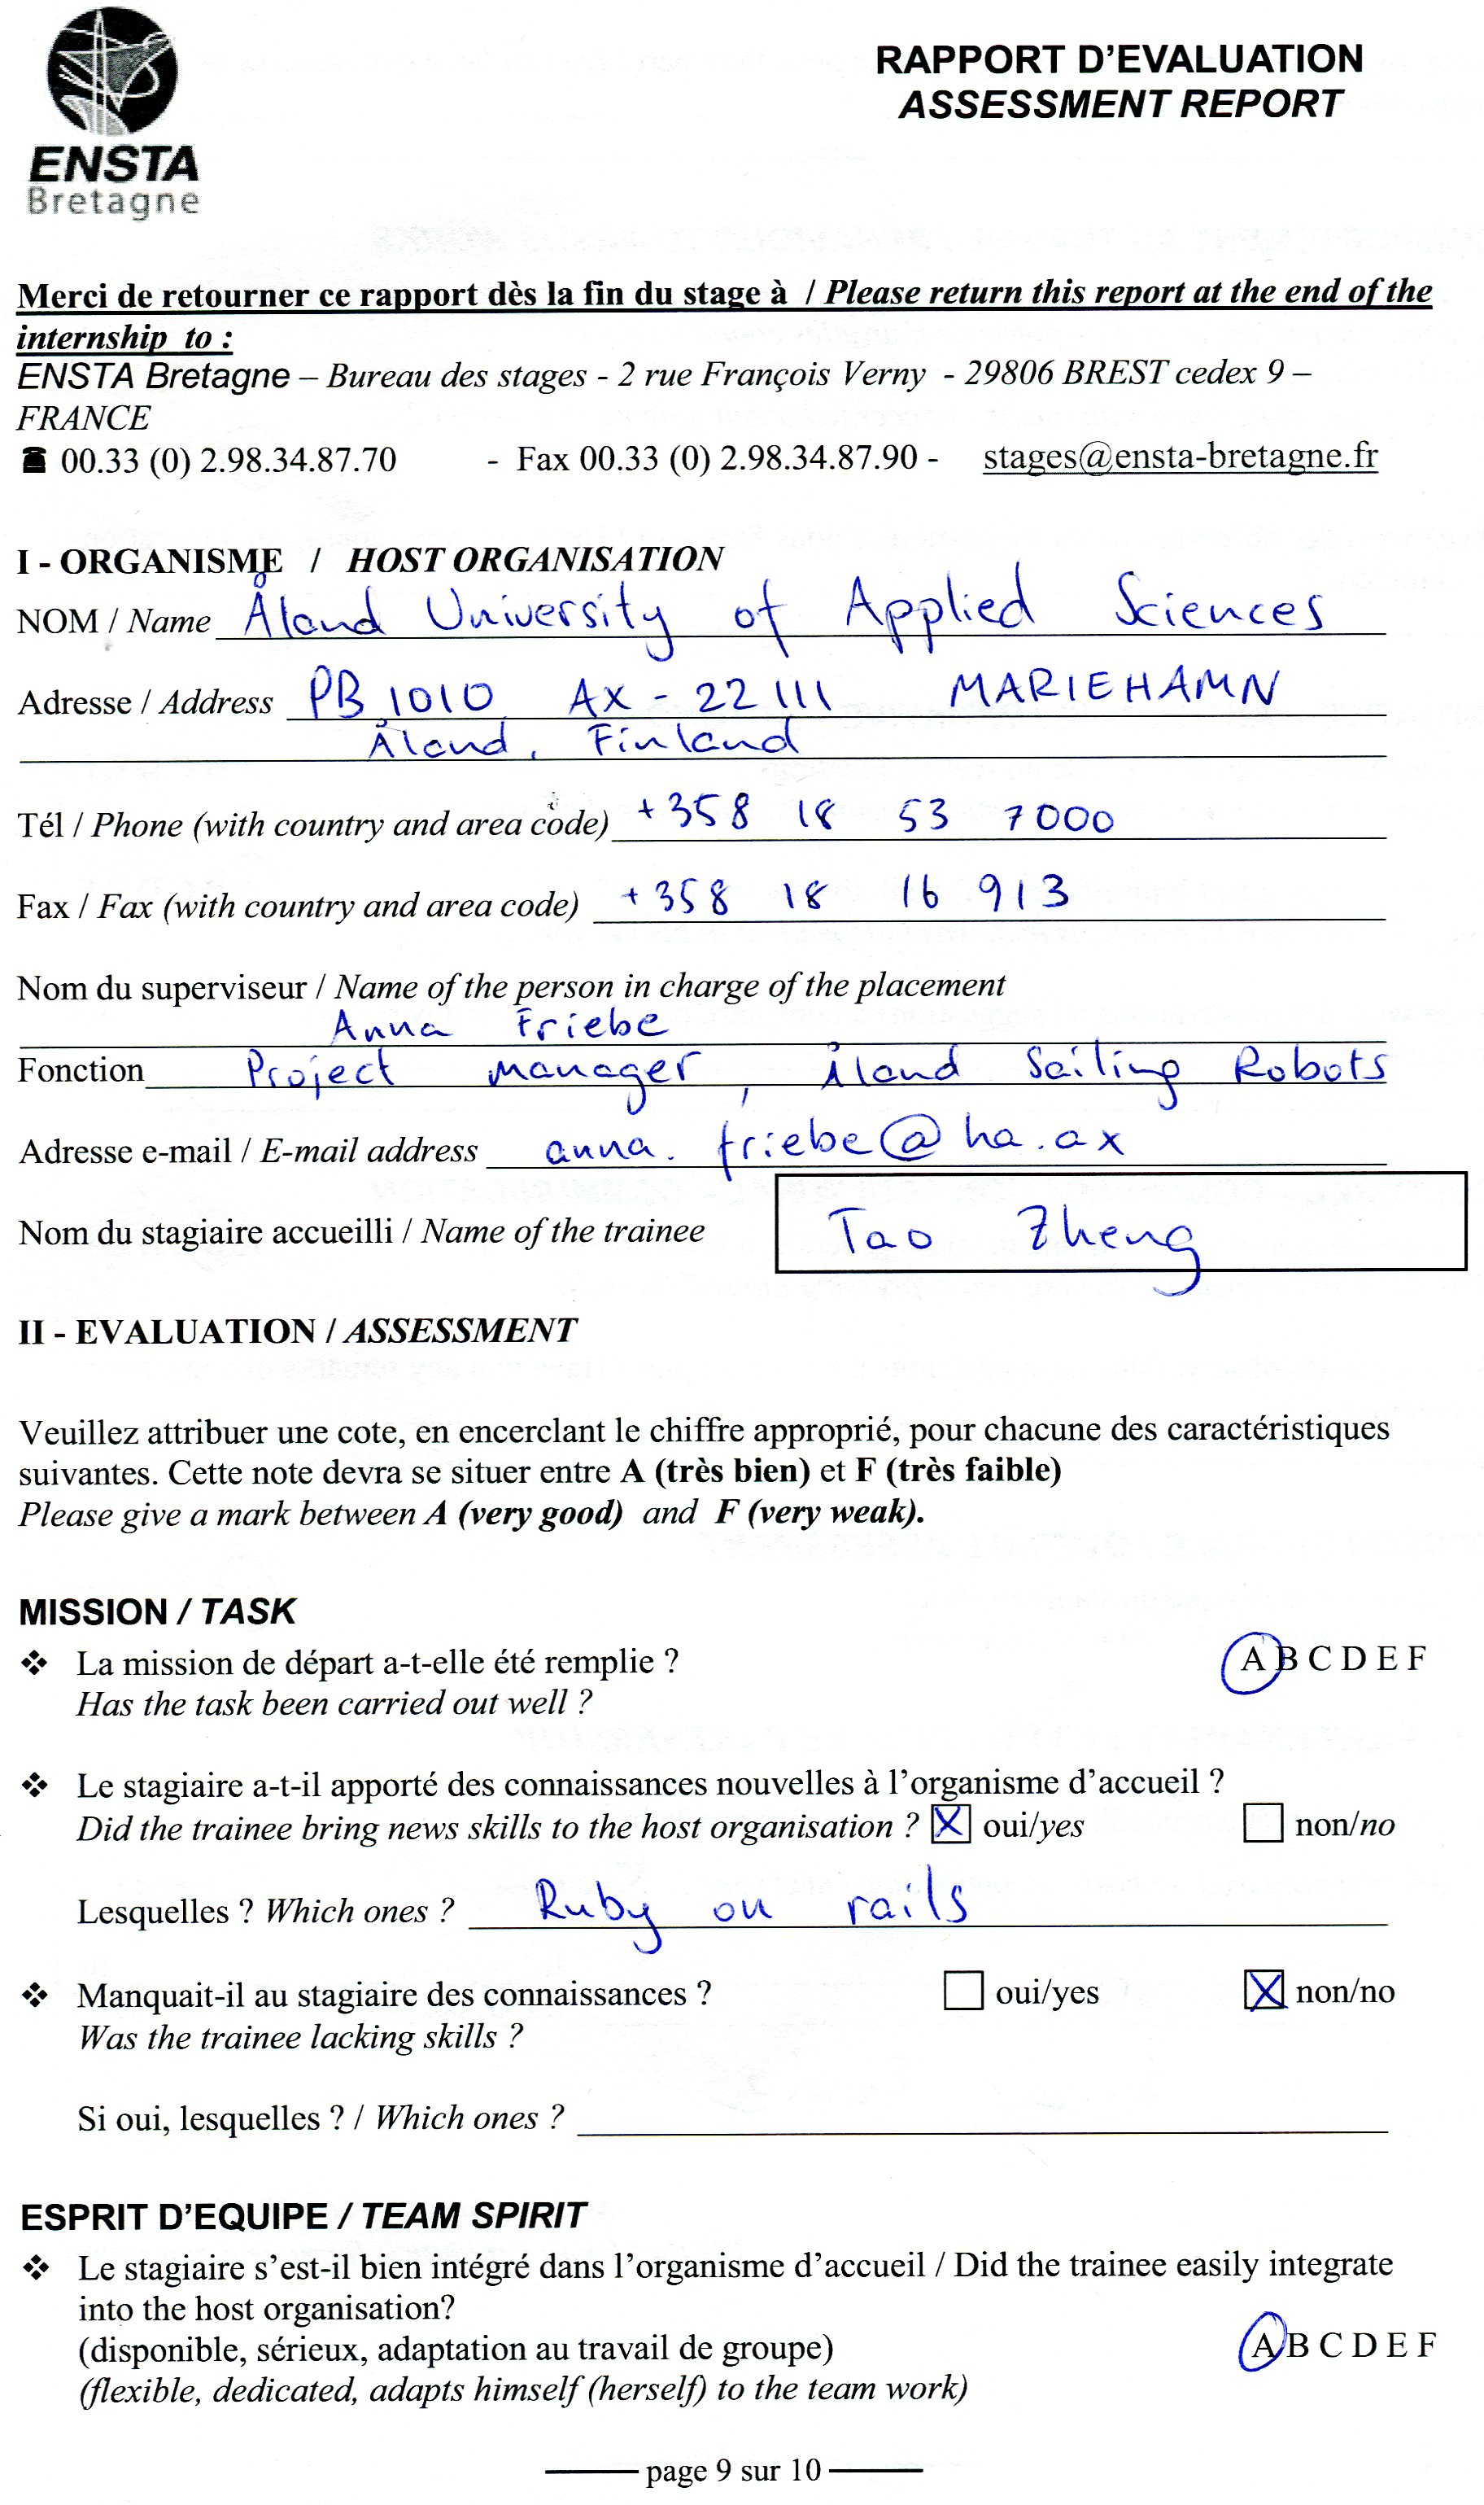
\includegraphics[width=12cm]{verso.jpg}
    \label{fig-sample}
\end{figure}
\begin{figure}[h!]
    \centering
    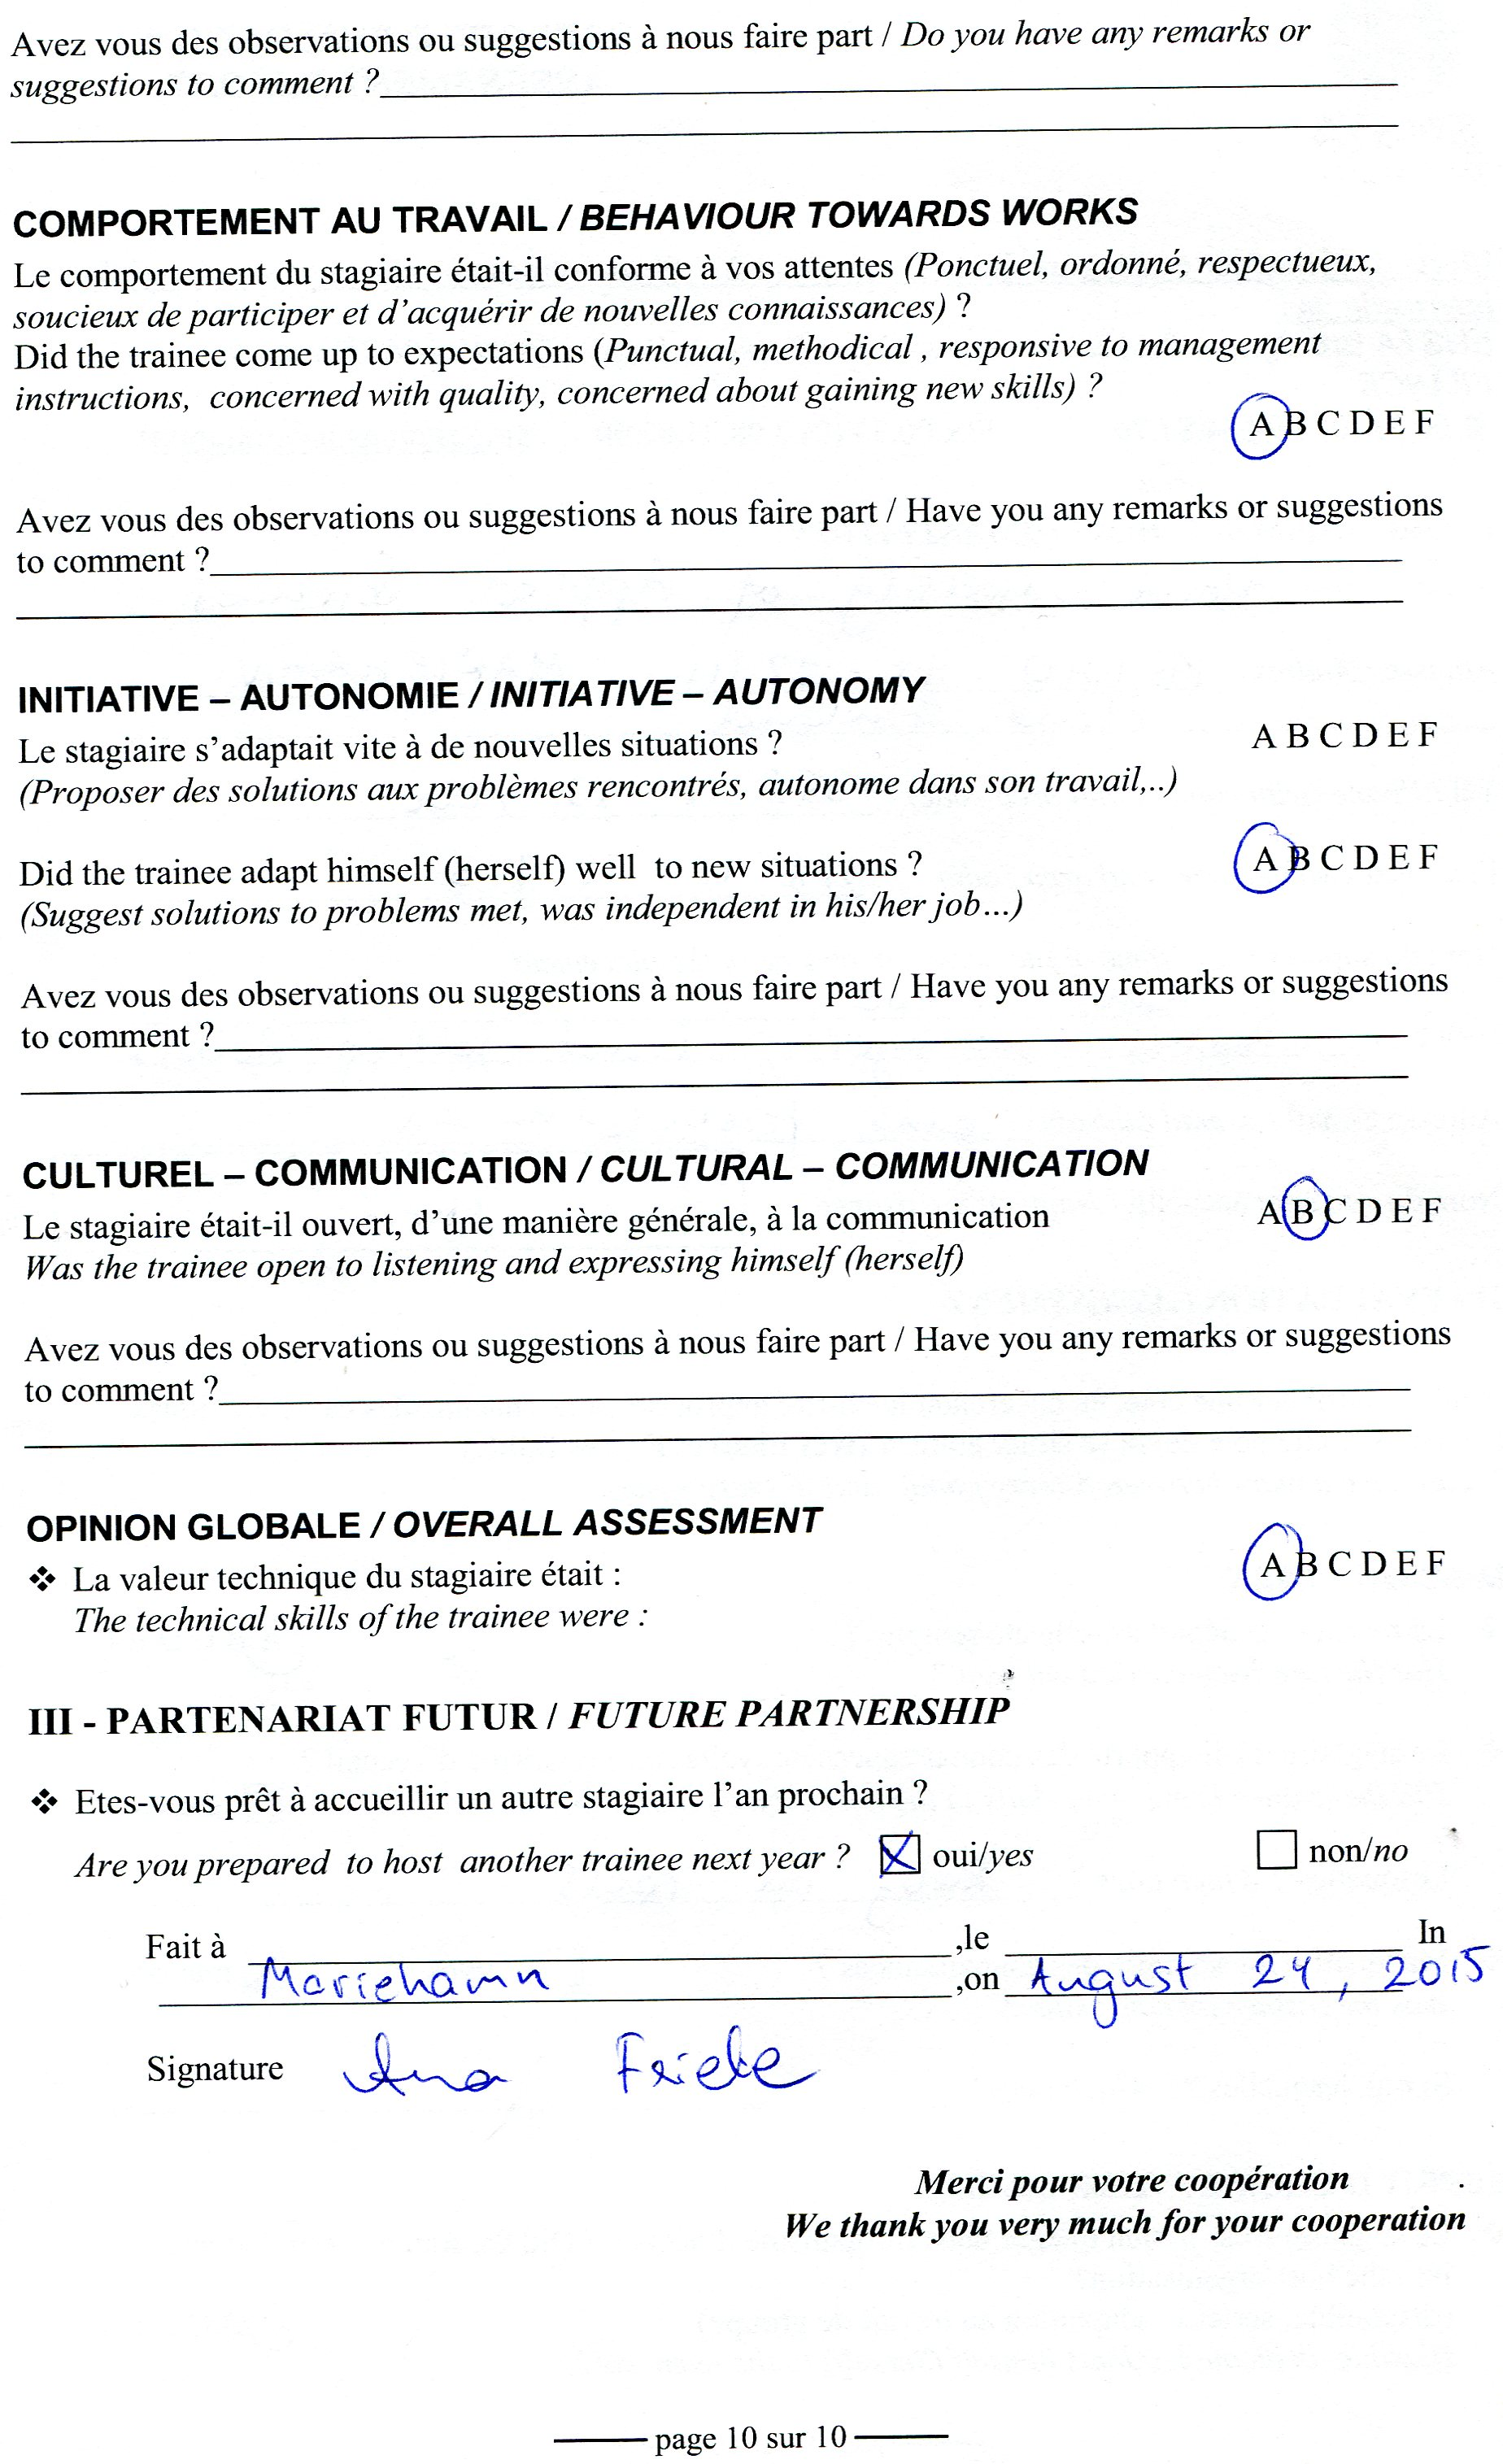
\includegraphics[width=12cm]{recto.jpg}
    \label{fig-sample}
\end{figure}